\documentclass[conference]{IEEEtran}
\IEEEoverridecommandlockouts
% The preceding line is only needed to identify funding in the first footnote. If that is unneeded, please comment it out.
\usepackage{cite}
\usepackage{amsmath,amssymb,amsfonts}
\usepackage{algorithmic}
\usepackage{graphicx}
\usepackage{textcomp}
\usepackage{xcolor}
\usepackage{hhline}
\def\BibTeX{{\rm B\kern-.05em{\sc i\kern-.025em b}\kern-.08em
    T\kern-.1667em\lower.7ex\hbox{E}\kern-.125emX}}
\begin{document}

\title{An Efficient and Implementation-friendly Method of Precision-adaptive Column-parallel ADC Design for More Intelligent Edge Computing\\}
%An Efficient and Implementation-friendly ADC extension Method with Precision Adaptive and Fine-grained Power Management Strategies for More Intelligent Edge Computing Scenarios

\author{\IEEEauthorblockN{1\textsuperscript{st} Given Name Surname}
\IEEEauthorblockA{\textit{dept. name of organization (of Aff.)} \\
\textit{name of organization (of Aff.)}\\
City, Country \\
email address or ORCID}
\and
\IEEEauthorblockN{2\textsuperscript{nd} Given Name Surname}
\IEEEauthorblockA{\textit{dept. name of organization (of Aff.)} \\
\textit{name of organization (of Aff.)}\\
City, Country \\
email address or ORCID}
\and
\IEEEauthorblockN{3\textsuperscript{rd} Given Name Surname}
\IEEEauthorblockA{\textit{dept. name of organization (of Aff.)} \\
\textit{name of organization (of Aff.)}\\
City, Country \\
email address or ORCID}
\and
\IEEEauthorblockN{4\textsuperscript{th} Given Name Surname}
\IEEEauthorblockA{\textit{dept. name of organization (of Aff.)} \\
\textit{name of organization (of Aff.)}\\
City, Country \\
email address or ORCID}
\and
\IEEEauthorblockN{5\textsuperscript{th} Given Name Surname}
\IEEEauthorblockA{\textit{dept. name of organization (of Aff.)} \\
\textit{name of organization (of Aff.)}\\
City, Country \\
email address or ORCID}
\and
\IEEEauthorblockN{6\textsuperscript{th} Given Name Surname}
\IEEEauthorblockA{\textit{dept. name of organization (of Aff.)} \\
\textit{name of organization (of Aff.)}\\
City, Country \\
email address or ORCID}
}

\maketitle

\begin{abstract}

Deploying Neural Networks (NNs) on edge devices is an emerging trend which leads to many efforts of research, where improving the system's energy efficiency is critical.
While the the NNs have been able to process data of varying precision for more efficient multi-task analysis, Analog-to-Digital Converters (ADCs), 
which dominate the power consumption of traditional sensing systems, can also be smartly designed for more intelligent edge computing. 
In this work, we focus on the column-parallel ADCs which are widely applied in the image processing applications and Compute-in-Memory (CIM) architecture, and 
an efficient and implementation-friendly method of the precision-adaptive column-parallel ADC design is proposed with fine-grained power gating strategies.
We present two case study ADC designs applied in CMOS Image Proceessors (CISs) and demonstrate the effectiveness of the proposed method in detail. 
Results show that almost a half of the ADCs’ power consumption can be saved for low-precision conversion, while just a few of extra control circuits is required.

\end{abstract}

\begin{IEEEkeywords}

ADC, precision-adaptive, energy-efficient, edge computing

\end{IEEEkeywords}

\section{Introduction}

With the development of the Internet-of-Things (IoT), edge devices like mobile phones, smart watches, and other portable products have been playing an important role in people’s daily lives 
for collecting and processing data in site and in time. On the other hand, Neural Networks have shown broad prospects for sensing applications, such as computer vision, speech recognition, 
and robotics. Therefore, deploying NNs on edge devices is an emerging trend which leads to many efforts of research. 

To integrate large and computationally intensive NN models on edge devices of which the power supply and computing resources are quite limited, improving the systems' energy efficiency is critical. 
While precision-compressed NN models \cite{leibe_xnor-net_2016}\cite{Ternary Weight Networks}\cite{park_energy-efficient_2018} and implementation with CIM architecture \cite{chiu_4-kb_2020}\cite{karunaratne_-memory_2020}\cite{jung_crossbar_2022} have been extensively studied, Analog-to-Digital Converters, which dominate the power consumption of 
traditional sensing systems, can also be precision-adaptively designed for more intelligent edge computing.
%can also be smartly designed for more intelligent edge computing. 

%As the NN models have been able to process data of varying precision for efficient multi-task analysis [xxxx], opportunities have been offered for us to further improve 
%the systems' energy efficiency by taking algorithm-aware adjustments inside the ADCs. Considering the precision (i.e. the quantization bits) is at the heart of an ADC’s energy constraints, 
%making it dynamically adaptive will be promising.

There have been related works on precision-configurable ADC design \cite{xia_10-bit_2006}\cite{zhu_06_2013}\cite{zhu_6--10-bit_2015}. However, these works mainly focus on a single Successive Approximation Register (SAR) or pipeline ADC with complex extra control logic,
which is not suitable for image processing applications and CIM architecture where high throughput is required thus the ADCs are usually in the column-parallel style and the Single-Slope(SS)
conversion logic is widely adopted to avoid overhead of area and power.

Other works have dynamically adjusted the the camera’s resolution or clock frequency for more efficeient image processing \cite{lubana_digital_2018}\cite{likamwa_energy_2013}, where the precision of ADCs has not been considered as a variable. 
Besides, there are efforts trying to relieve the design specifications of ADCs by applying low-precision analog computing (whether with CIM architecture or not) firstly close to the sensor \cite{likamwa_redeye_2016}\cite{chen_asp_2016}\cite{liu_ns-cim_2020}. 
But high-precision ADCs and NN processors are still there for complex tasks. Therefore, taking algorithm-aware adjustments inside ADCs remains competitive.

Motivated by these facts, we mainly makes the following contributions in this paper:

\begin{enumerate}[\IEEEsetlabelwidth{3)}]
	\item 
	Two case study ADC designs applied in the CISs are presented with different design specifications. 
	The first one is column-parallel SS ADCs \cite{snoeij_18v_2005}\cite{kleinfelder_10000_2001} and the second is column-parallel SAR/SS ADCs \cite{kim_area-efficient_2016}.
	Both of the two designs are built completely with not only main functional modules but also bandgap circuits, bias circuits and necessary buffers.
	\item 
	We analyse the power distribution across all related circuits of the ADCs, according to which a method combining adaptive precision and fine-grained power gating strategies is proposed
	for more samrt data conversion.  
	And the effectiveness of this method is demonstrated with specific simulating results, showing that the ADCs' power consumptionin can be reduced to nearly half for low-precision conversion.  
	\item 
	Although with different details, we apply this method successfully to the two different ADC designs with the same principles and just a few of extra control circuits are required.
	Therefore, we argue for the universality of the proposed method.
\end{enumerate} 

The remainder of this paper is organized as follows. 
Sect.~\ref{architecture} presents the architecture overview of the two case study ADC designs. 
Sect.~\ref{strategy} describes the implementation of the proposed method for the two case study ADC designs. 
Sect.~\ref{result} reports the evaluation results and Sect.~\ref{discussion} develops discussions. 
Finally, Sect.~\ref{conclusion} concludes this paper.

\section{Architecture Overview}\label{architecture}

\subsection{Architecture of the SS ADCs}

The overall architecture of the SS ADCs is presented in Fig.~\ref{SSADC}. The main modules include column-parallel Correlated Double Sampling (CDS) circuits, comparators, 
and a column-shared ramp generator. Fig.~\ref{SSWAVE} shows the basic operational waveform of the SS ADCs. At the time when the ramp signal exceeds the output of a CDS circuit in a certain column, 
the corresponding comparator will be flipped and latch the time information $\Delta t$ in the 8-bit registers in that column as conversion results. 
And Such conversions across all columns will be done as soon as the ramp signal reaches $V_{refh}$.

\begin{figure}[htbp]
	\centerline{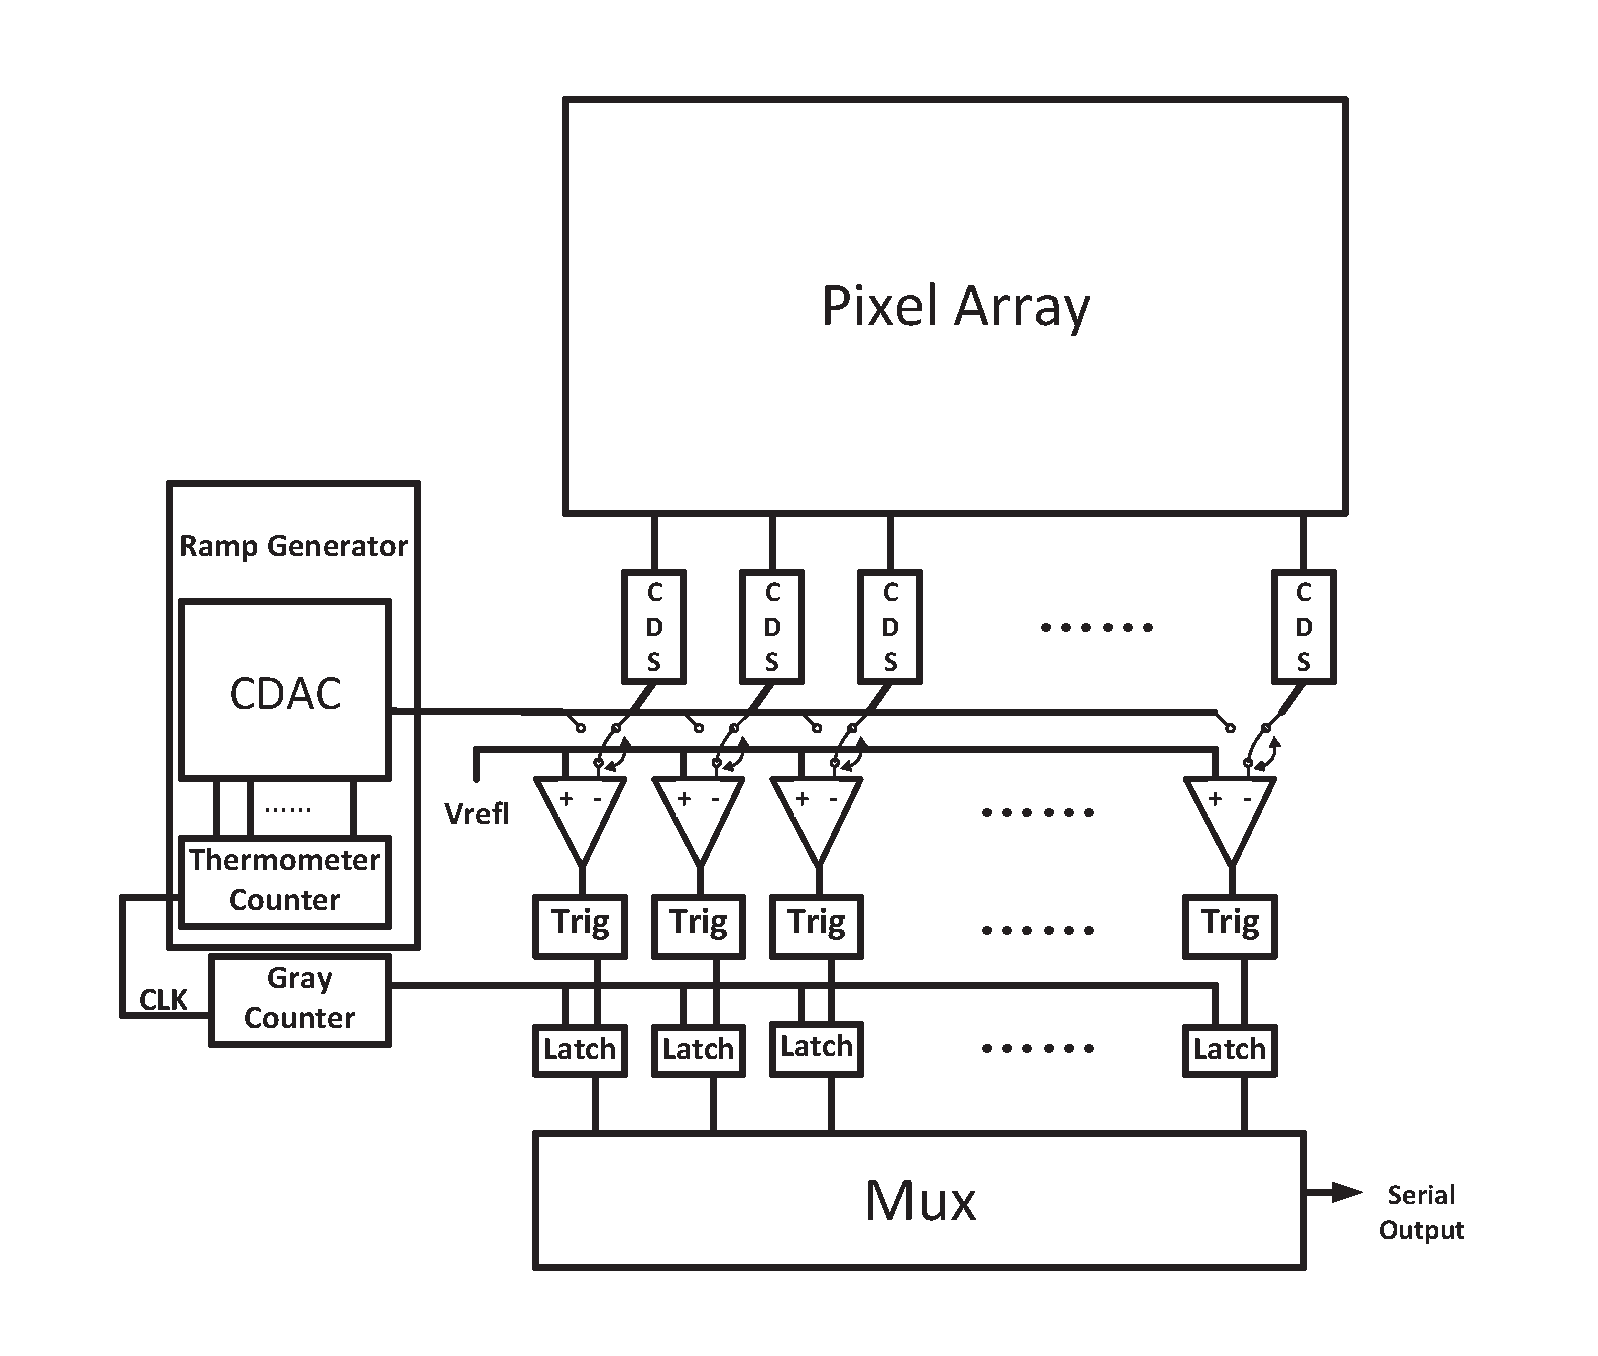
\includegraphics[width=3.5in]{./Figures/SSADC.eps}}
	\caption{Overall Architecture of the SS ADCs.}
	\label{SSADC}
\end{figure} 

\begin{figure}[htbp]
	\centerline{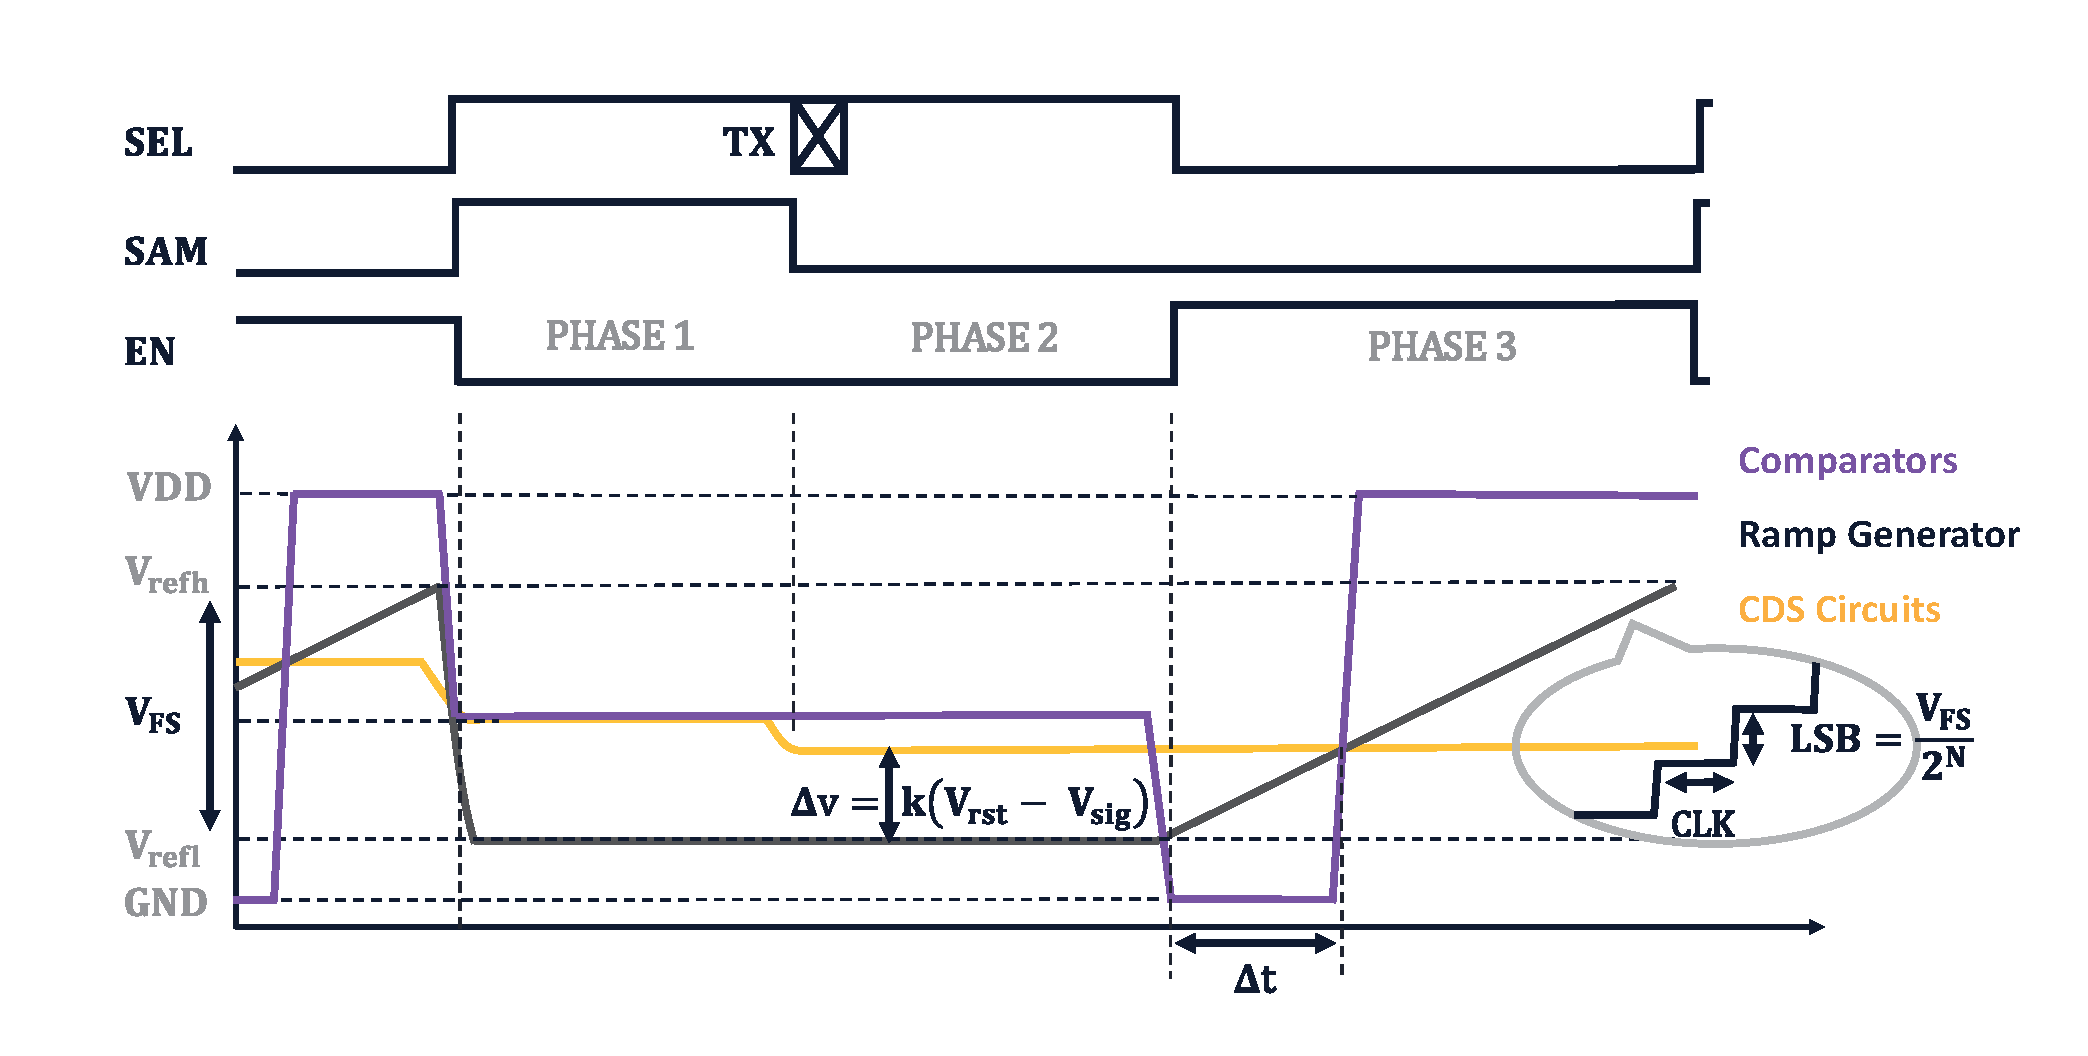
\includegraphics[width=3.5in]{./Figures/SSWAVE.eps}}
	\caption{Operational waveform of the SS ADCs.}
	\label{SSWAVE}
\end{figure}

As the structure of the three main modules are described more specifically as follows, details of the three waves in Fig.~\ref{SSWAVE} are also revealed.

\subsubsection{CDS Circuits}

CDS circuits are the interface between the pixel array and the ADCs, responsible for subtracting the pixels’ signal voltages from reference voltages and 
amplifying the difference by a certain coefficient. The difference (i.e. $\Delta{V}$ in Fig.~\ref{SSWAVE}) is physically attached to the exposure time of the pixels, 
and the subtraction will help cancel the noises caused by the varying reference voltages. 

Switched-capacitor operational amplifiers are commonly used in CDS circuits as presented in Fig.~\ref{CDS}. According to the law of charge conservation, 
the output voltage of the CDS circuits (in PHASE2 of Fig.~\ref{SSWAVE}) can be calculated as \eqref{eq1}. It is noticed that the Input Offset Cancelation (IOS) is realized \cite{razavi_design_1992}, 
which is necessary because the amplifiers in different columns may have different offset voltage.

\begin{figure}[htbp]
	\centerline{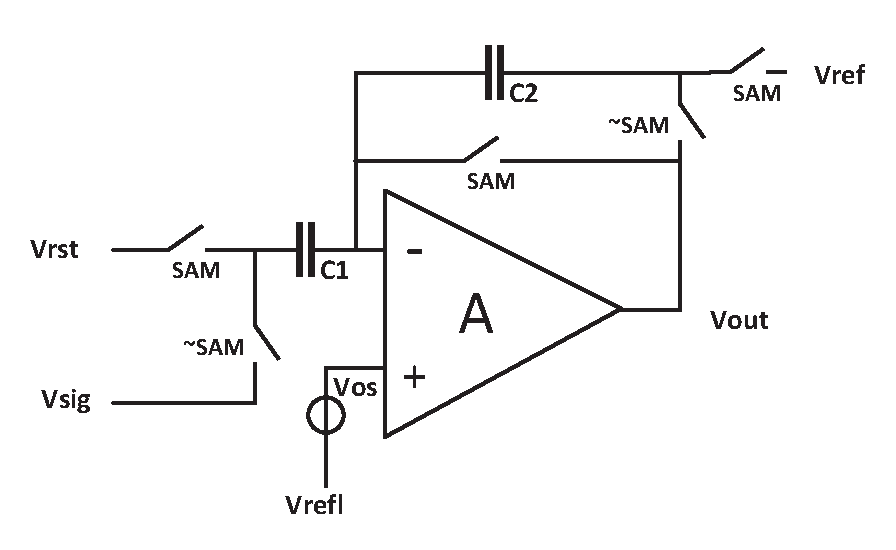
\includegraphics[width=2.5in]{./Figures/CDS.eps}}
	\caption{the Structure of the CDS Circuits.}
	\label{CDS}
\end{figure} 

\begin{equation}
\begin{aligned}
	V_{out}&=\left[ V_{ref}+\frac{C_1}{C_2}\ast\left(V_{rst}-V_{sig}\right)\right]\ast\frac{\beta A}{1+\beta A}\\
	 &\;{+}\;\left(V\right._{refl}+V_{os})\ast\frac{A}{1+A}\ast\frac{1}{\beta A}\\
	 &\;where\ \ \beta=\frac{C_2}{C_1+C_2}
	\label{eq1}
\end{aligned}
\end{equation}

\subsubsection{the Ramp Generater}

As presented in Fig.~\ref{RAMP}, the ramp generator consists of a thermometer counter and a Capacitor Digital-to-Analog Converter (CDAC). 
While the capacitors in CDAC are being switched one by one from $V_{refl}$ to $V_{vefh}$, the output voltage of the ramp generator will be as \eqref{eq2} according to the law of charge conservation. 
In this equation, $N$ means the number of switched capacitors and $M$ means the total number of capacitors of the same size (for the 8-bit precision, the total number will be 255). 
Therefore, as in PHASE3 of Fig.~\ref{SSWAVE}, the ramp signal will be like stages from $V_{refl}$ to $V_{refh}$, of which the range is consistent with the output of CDS circuits. 
And the height of every stage is actually the Least Significant Bit (LSB) converted by the ADCs.
 
The three buffers in Fig.~\ref{RAMP} make sure that the reference voltages and ramp signal have enough driving capability, 
and the output buffer will be in the largest size because it has to drive hundreds of column-parallel comparators.

\begin{figure}[htbp]
	\centerline{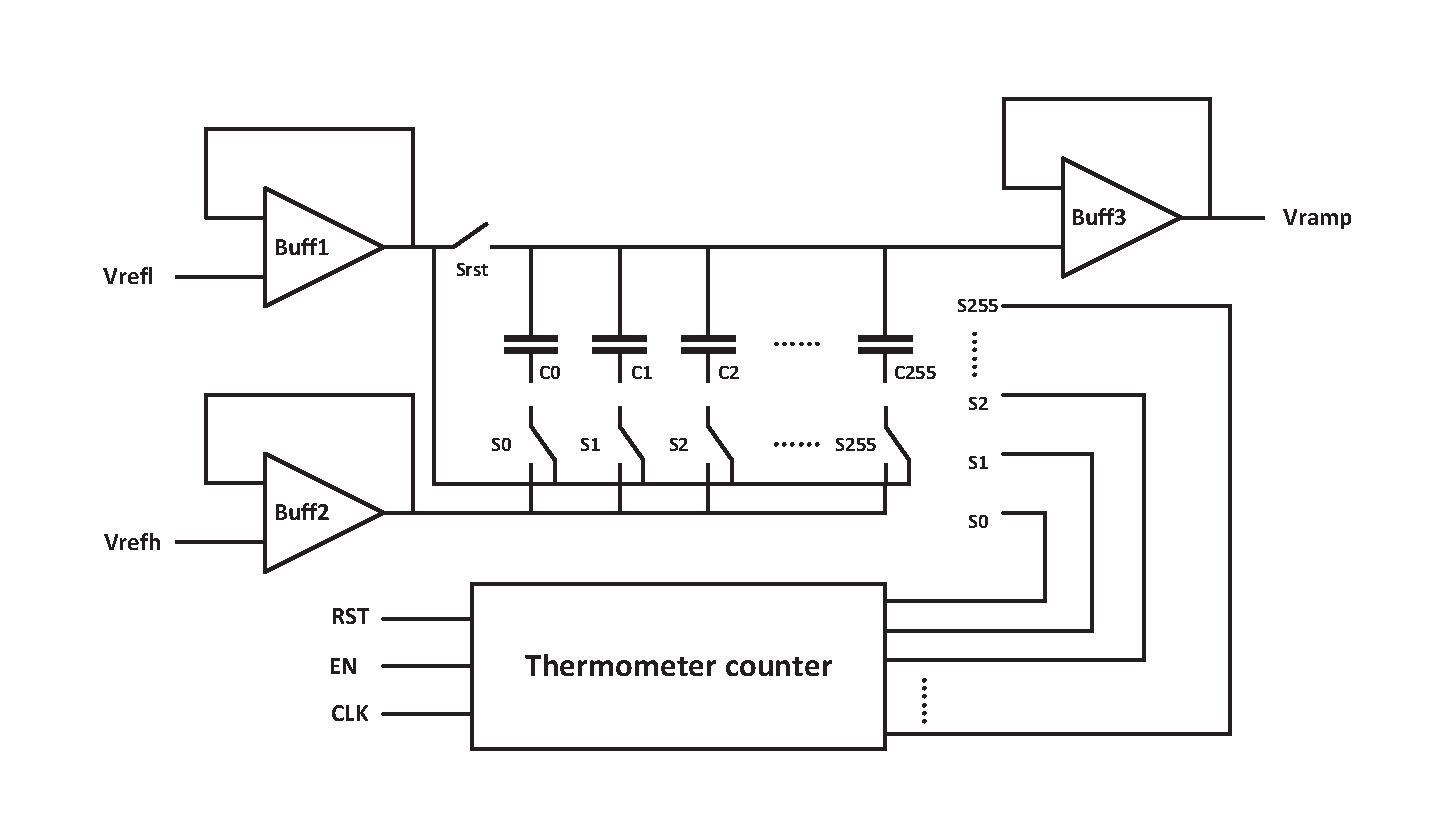
\includegraphics[width=3.5in]{./Figures/RAMP.eps}}
	\caption{the Structure of the Ramp Generator in the SS ADCs.}
	\label{RAMP}
\end{figure} 

\begin{equation}
	V_{ramp}=V_{refl}+\frac{N}{M}\ast\left(V_{refh}-V_{refl}\right)
		\label{eq2}
\end{equation}

\subsubsection{Comparators}

The comparators work for comparing the CDS circuits' output and the ramp signal from the ramp generator. 
In the SS ADCs, two-stage open-loop comparators can be applied as presented in Fig.~\ref{COM}. Again according to the law of charge conservation, 
the comparators’ output (in PHASE3 of Fig.~\ref{SSWAVE}) can be calculated as \eqref{eq3}. The comparison will be dominated by $V_{ramp}-V_{cds}$ as long as the amplifiers’ open-loop gain 
is large enough and the IOS is realized. Besides, the comparators’ speed depends on the amplifiers’ bandwidth and slew rate.

\begin{figure}[htbp]
	\centerline{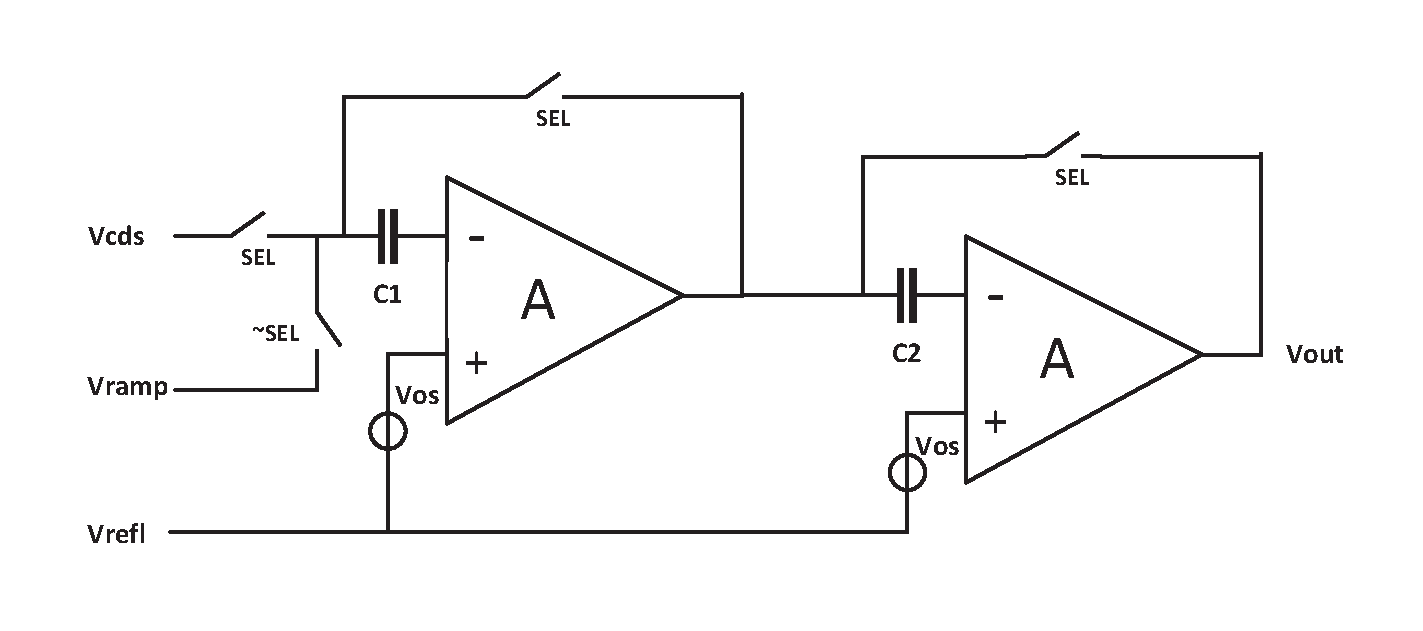
\includegraphics[width=3.5in]{./Figures/COM.eps}}
	\caption{the Structure of the Comparators in the SS ADCs.}
	\label{COM}
\end{figure} 

\begin{equation}
	\begin{aligned}
		V_{out}&=A^2(V_{ramp}-V_{cds})\\
		&\;{+}\;\left(V_{refl}+V_{os}\right)\ast\frac{A}{1+A}\\ 		
		\label{eq3}
	\end{aligned}
\end{equation}

\subsection{Architecture of the SAR/SS ADCs}

The overall architecture of the SAR/SS ADCs is almost the same as the SS ADCs, and the only two differences are that the comparators are replaced by low-precision (4bit) SAR sub-ADCs and
the ramp generator is replaced by a Resistor Digital-to-Analog Converter (RDAC) with a one-hot counter.

As presented in Fig.~\ref{SAR}, while the SAR sub-ADCs generating the upper 4-bit results, $V_{X}$ in Fig.~\ref{SAR} will be changed according to SAR logic. That means after 4 comparisons 
with the reference voltage, $V_{X}$ will be as \eqref{eq4}, where $D_{U}\left[\,i\,\right]$ is the $i$ th bit of the upper 4 bits. We assign 14 steps for the 4 comparisons with SAR logic, 
and then the ramp generator will start working, making $V_{X}$ increase gradually as \eqref{eq5}, where $D_{L}\left[\,i\,\right]$ is the $i$ th bit of the lower 6 bits. 
At the time when $V_{X.2}$ exceeds $V_{ref}$, the corresponding $V_{cds}$ will be as \eqref{eq6}, represented by the 10-bit conversion results, exactly.

Fig.~\ref{RRAMP} shows the structure of the ramp generator in the SAR/SS ADCs, which consists of an R-string made up of 68 unit resistors. $V_{ramp}$ has a total number of 68 steps,
of which 64 steps with a step size of $(V_{refh}-V_{refl})/64$ are used to generate the lower 6-bit results and 4 steps are used to make sure that the comparators 
will always be flipped for lacthcing the results. In the working time, $V_{0}$ to $V_{67}$ in the ramp generator is sequentially selected as the input of the output buffer and thereby 
$V_{ramp}$ is changed from $V_{vefl}$ to $V_{vefl}+17/16(V_{refh}-V_{refl})$.

Compared to CDAC, RDAC is able to generate the ramp signal without the gain error caused by the input capacitors of the output buffer, 
which is necessary for achieving 10-bit precision in the SAR/SS mixed architecture.
Besides, the two buffers of the reference voltages in the RDAC require less energy than those in the CDAC due to less load capacitance.  

The related operational waveform of the SAR/SS ADCs is presented in Fig.~\ref{SARWAVE}. It is obvious that the upper 4-bit results (as the second last item of \eqref{eq6}) are generated 
with the SAR logic and the lower 6-bit results (as the last item of \eqref{eq6}) is counted according to the time between the ramp signal’s start and the comparators’ last flip. 

\begin{figure}[htbp]
	\centerline{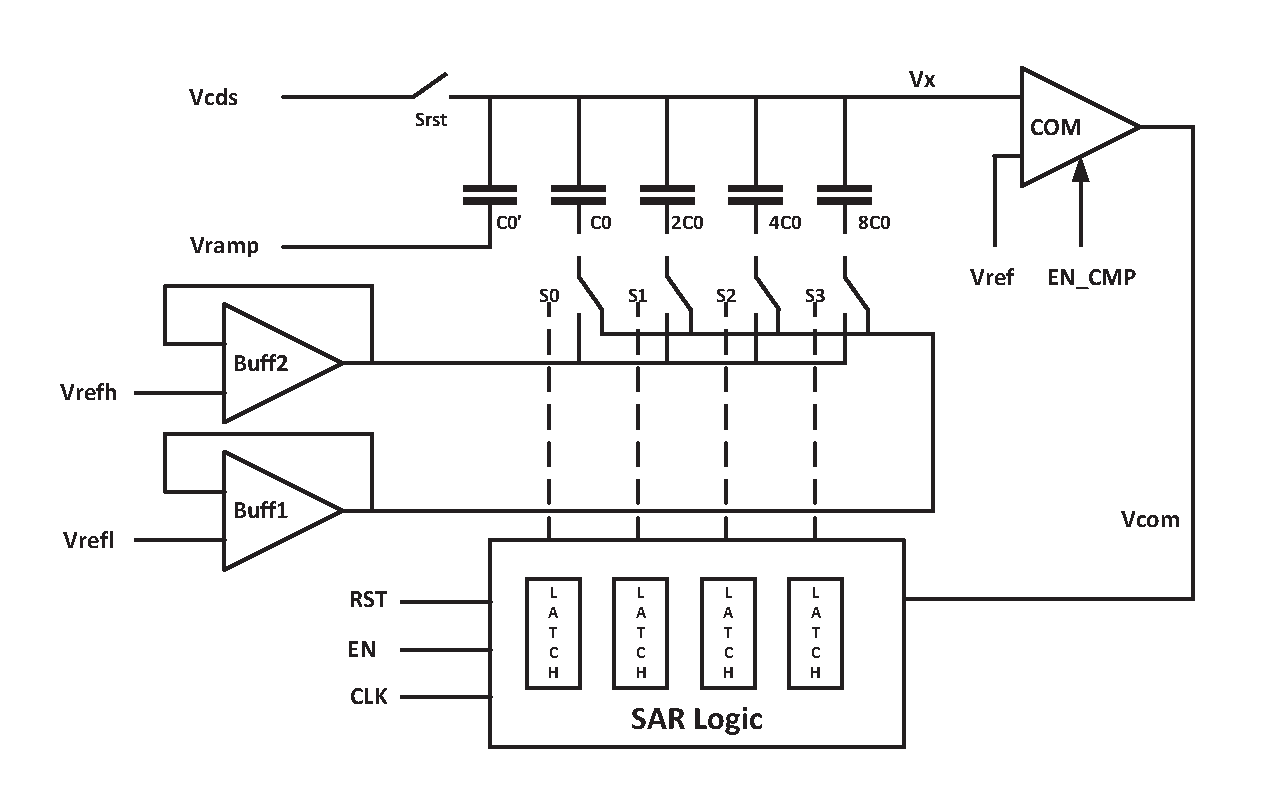
\includegraphics[width=3.5in]{./Figures/SAR.eps}}
	\caption{the Structure of the SAR Sub-ADCs in the SAR/SS ADCs.}
	\label{SAR}
\end{figure}

\begin{figure}[htbp] 
	\centerline{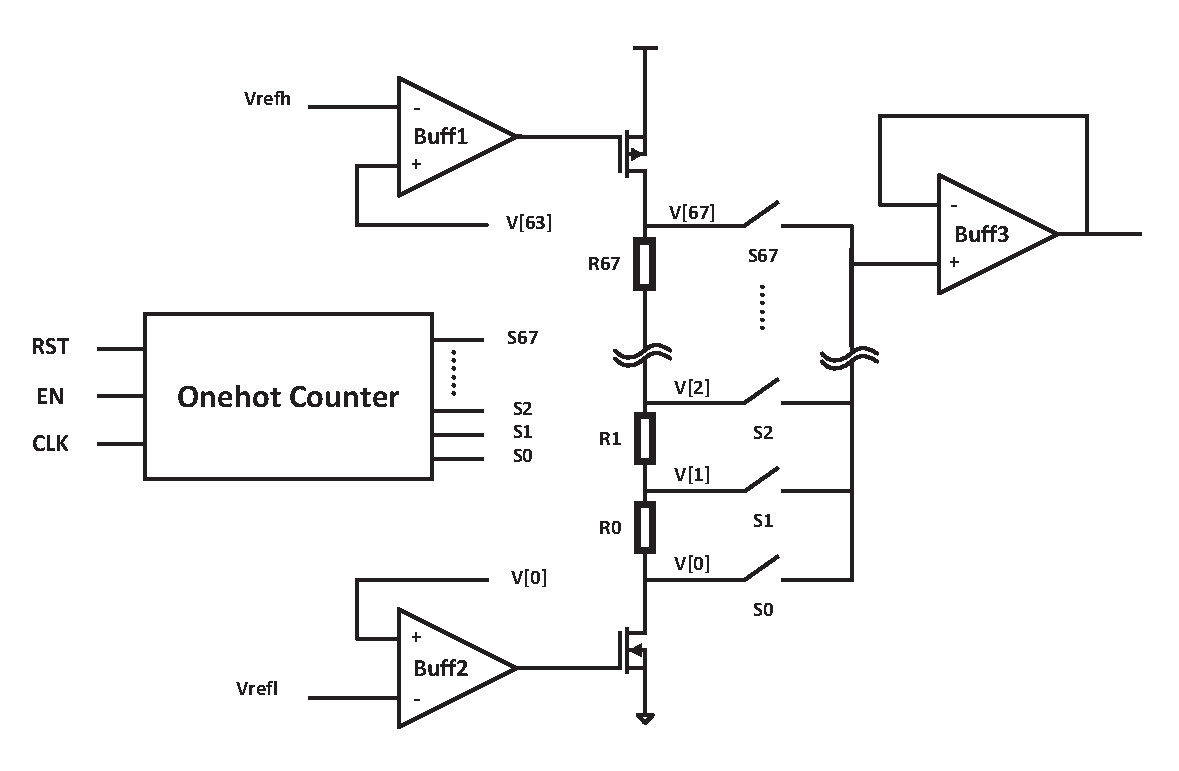
\includegraphics[width=3.5in]{./Figures/RRAMP.eps}}
	\caption{the Structure of the Ramp Generator in the SAR/SS ADCs.}
	\label{RRAMP}
\end{figure} 

\begin{equation}
	V_{X.1}=V_{cds}+\sum_{i=1}^{4} {\frac{V_{ref}}{2^{i}}\ast{D_{U}\left[\,i\,\right]}}
	\label{eq4}
\end{equation}

\begin{equation}
	\begin{aligned}
	&V_{X.2}=V_{X.1}+\frac{V_{ramp}}{2^4}\\ &where\  V_{ramp}=\frac{V_{ref}}{2^6-1}\ast\sum_{i=1}^{6}2^{6-i}\ast{D_{L}\left[\,i\,\right]}
	\label{eq5}
	\end{aligned}	
\end{equation}

\begin{equation}
	\begin{aligned}
	V_{cds}&=k\ast(V_{rst}-V_{sig})\\
	&\;{\approx}\;{V_{ref}-\sum_{i=1}^{4} \frac{V_{ref}}{2^{i}}\ast{D_{U}\left[\,i\,\right]}-\sum_{i=1}^{6} \frac{V_{ref}}{2^{4+i}}\ast{D_{L}\left[\,i\,\right]}}
	\label{eq6}
	\end{aligned}
\end{equation}

\begin{figure}[htbp]
	\centerline{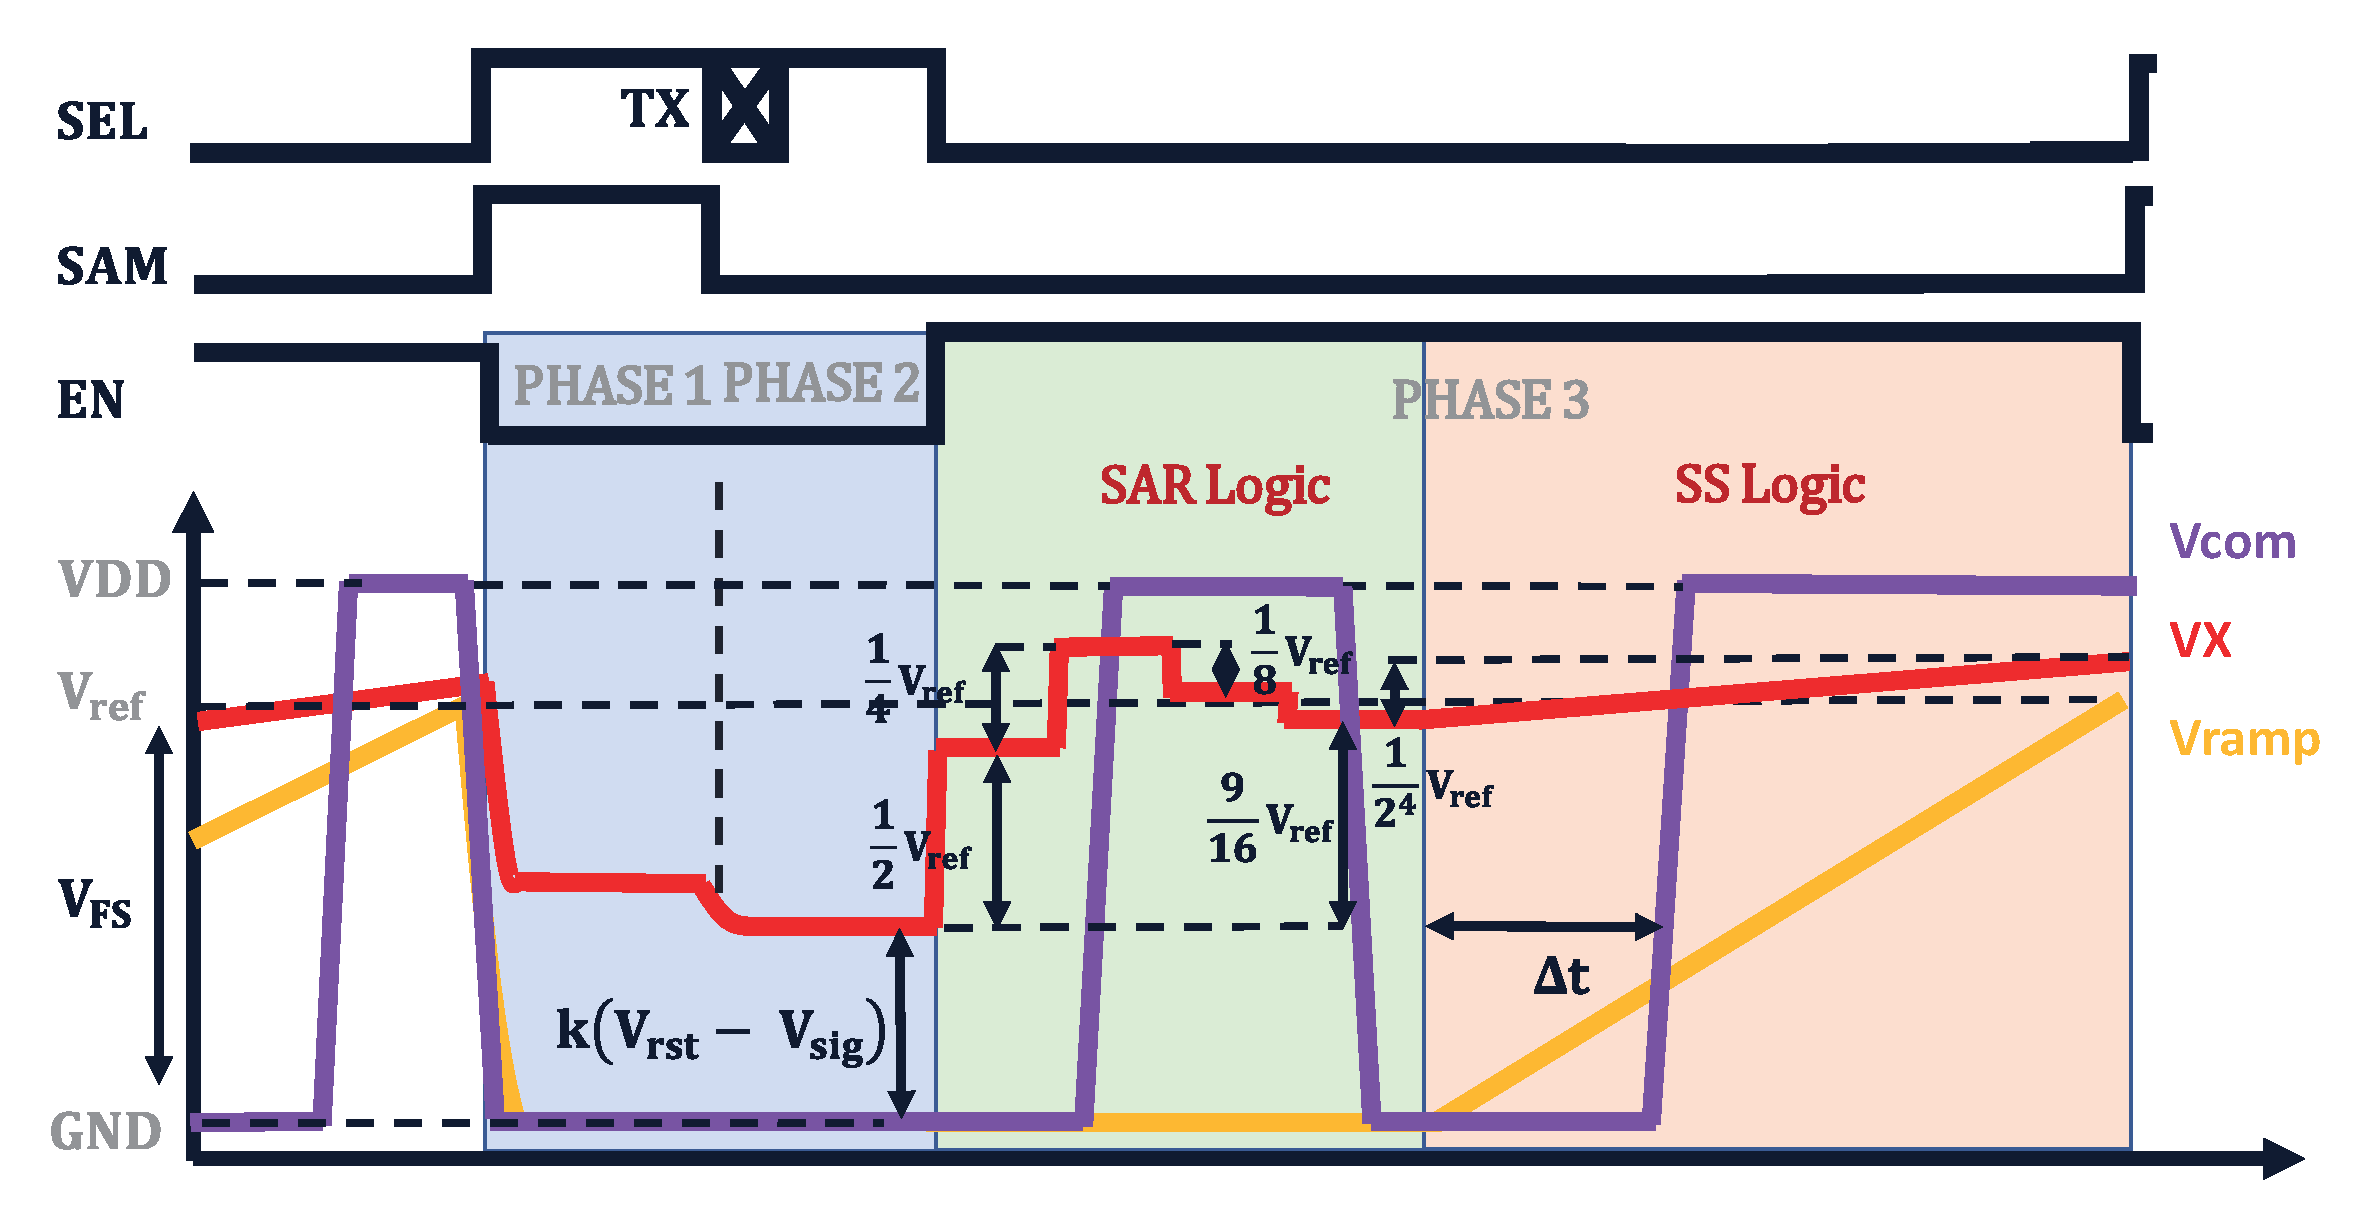
\includegraphics[width=3.5in]{./Figures/SARWAVE.eps}}
	\caption{the Structure of the SAR Sub-ADCs in the SAR/SS ADCs.}
	\label{SARWAVE}
\end{figure} 

As for the comparators inside the SAR sub-ADCs, traditional structure of a strong-arm comparator with pre-amplifiers is adopted as presented in Fig.~\ref{LATCH}. Such comparators 
are suitable for multiple comparisons because high speed is easy to achieve. Besides, the pre-amps’ offset voltages can be canceled effectively through the Output Offset Cancelation (OOS) \cite{razavi_design_1992}.

\begin{figure}[htbp]
	\centerline{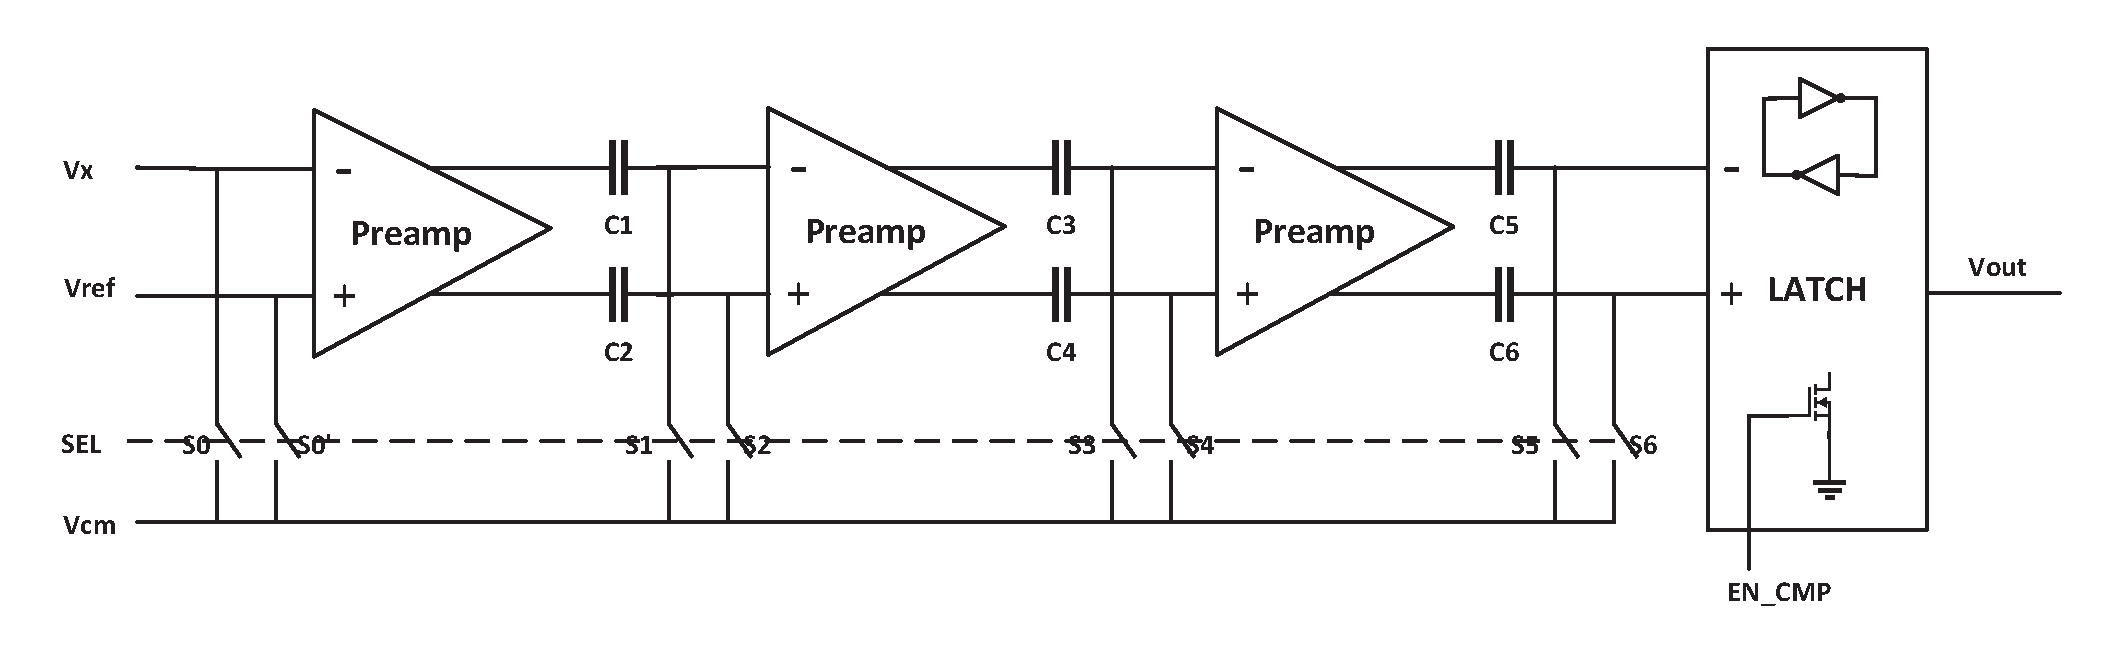
\includegraphics[width=3.5in]{./Figures/LATCH.eps}}
	\caption{the Structure of the Comparators in the SAR Sub-ADCs.}
	\label{LATCH}
\end{figure} 

 The total steps for conversion in the SAR/SS ADCs are 82 ($14+68$), which is much less than 1024 steps (for 10-bit) with the SS architecture. 
 However, the SAR/SS ADCs have traded off area for less conversion steps. Therefore, for different design specifications, different arcitecture can be chosen.

\section{Implementation of Adaptive Precision and Power Gating}\label{strategy}

\subsection{Power Gating Implementation}

The power gating can be implemented simply by adding PMOS-transistor switches between the functional blocks and the supply voltage \cite{keating_low_2007}. 
When the switches are turned off, the corresponding blocks’ current paths will be cut off, thus the energy is saved. 
It is obvious that the more currents are under control, the more effective the power gating can be. However, to avoid unacceptable IR drop, the total size of the switches may be large, 
thus inverters should be inserted between the control signal and the switches’ gates for adequate driving capability. 
Besides, the longer time the blocks can be power gated, the more energy can be saved. And a single long power off time is preferred than multiple short time for power gating because
the functional blocks’ recovery speed from power off should also be taken into consideration.

Power gating is efficient for the collumn-parallel ADCs because not only the sum of column-parallel currents that can be controled is large.
but also the widely adopted SS conversion logic offers rather long potential time for power off.
In addition, gating the buffers or amplifiers will cut off the paths for both static currents and dynamical charge currents. 

\subsection{Implementation for the SS ADCs}

As evaluated in Sect.~\ref{result}, the SS ADCs’ power consumption is mainly taken up by the column-parallel comparators, bias circuits, and the output buffer of the ramp generator. 
Considering that all bias circuits are settled down only once (tens of microseconds after the whole system's power up) and then other circuits can be settled down quickly by the distributed 
bias circuits, we just apply power gating to the amplifiers in the comparators and the output buffer in the ramp generator.

The related waveform are presented in Fig.~\ref{SS_pg}. For low-precision conversion, the thermometer counter should have been extended to support switching the capacitors in CDAC 16 by 16 
rather than one by one, thus the ramp signal will reach $V_{refh}$ in 16 steps (for 4 bits) rather than 256 steps (for 8 bits). After the 16 steps the comparators and the output buffer 
can be power gated for a long time leaving the output signals change freely.

\begin{figure}[htbp]
	\centerline{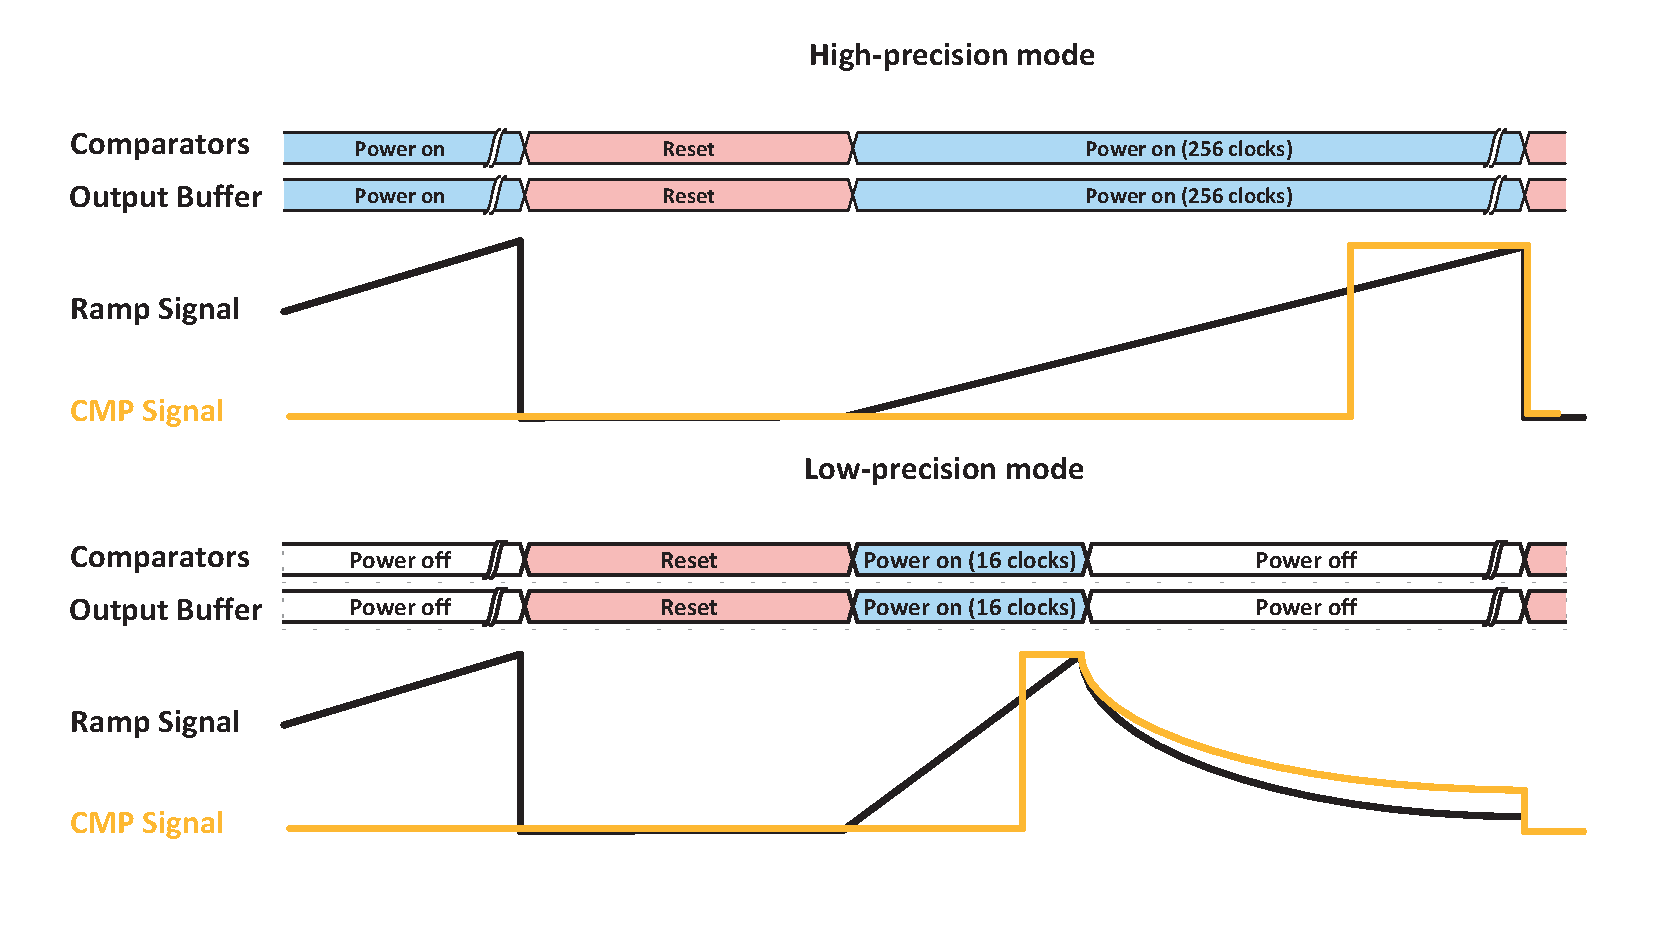
\includegraphics[width=3.5in]{./Figures/SS_pg.eps}}
	\caption{Power Gating and Adaptive Precision Strategies for the SS ADCs.}
	\label{SS_pg}
\end{figure} 

\subsection{Implementation for the SAR/SS ADCs}

As evaluated in Sect.~\ref{result}, the SAR/SS ADCs’ power consumption is mainly taken up by the column-parallel buffers of reference voltages in the SAR sub-ADCs.
It is because that these buffers need to drive relatively large and changing load capacitance, which means relatively large static and dynamical currents are required.
The waveform of related power gated signals is presented in Fig.~\ref{SAR_pg}. It is noticed that the comparators are also in control because they can conveniently share the same gating signal 
as the buffers and they do consume some energy. For low-precison conversion, the ramp signal is generated as usaual but the buffers and comparators will be power off, 
leaving the 4-bit results converted completely by the SAR logic. 

Compared with the SS ADCs, the one-hot counter in the SAR/SS ADCs does not need to support two modes for adaptive precision. 
Besides, the start signal of the ramp generator and the power off signal of the buffers can also be the same. Therefore, the SAR/SS ADCs relatively require less extra control circuits.
As for the proportion between the power off time and the conversion time, 64/78 is achieved in the SAR/SS ADCs, which is a little less than the number 240/256 in the SS ADCs.

\begin{figure}[htbp]
	\centerline{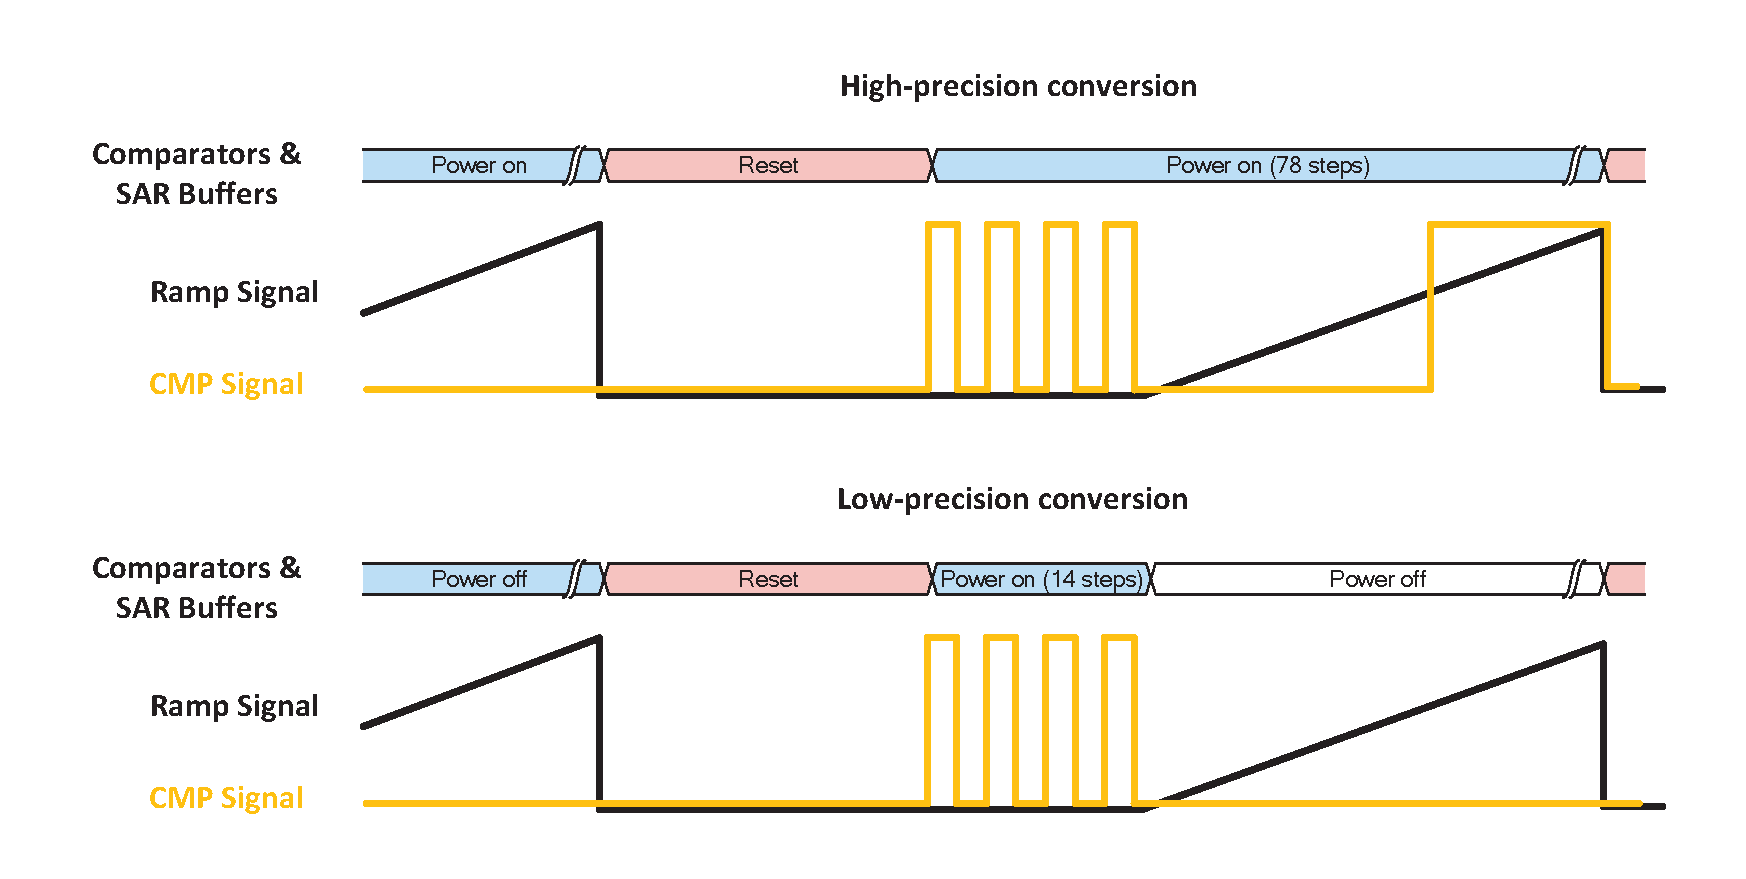
\includegraphics[width=3.5in]{./Figures/SAR_pg.eps}}
	\caption{Power Gating and Adaptive Precision Strategies for the SAR/SS ADCs.}
	\label{SAR_pg}
\end{figure} 

\section{Evaluation Results}\label{result}

This section provides quantitative results of the two case study ADC designs’ fundamental characteristics and energy-saving performance. 
The statistical data is obtained from simulation in Virtuoso’s AMS Environment. 
Although some digital modules are in behavior level written by Verilog, we argue that the power consumption of this parts can be ignored 
because these digital modules are just in need of limited dynamical currents.

\subsection{Evaluation of the SS ADCs}

The fundamental characteristics of the SS ADCs are summarized in Table~\ref{tab1}. Assuming a 512×512 pixel array, the frame rate will be 162fps.
The SNDR of SS ADCs is 23.83/46.64 dB, which means the ENOB is 3.67/7.46 bits. 
The power consumption of the SS ADCs is measured and divided by columns, 
it shows that compared to 76.2uW/column for high-precison conversion, only 40.8uW/column is needed for low-precison conversion, reduced by almost a half. 
A more specific energy analysis is presented in Fig.~\ref{SSresults1}. 
As we can see, most parts of the power consumption are taken up by the column-parallel comparators and output buffer of the ramp generator, 
both of which can be power gated effectively for low-precison conversion. 
The related quantity results is presented in Fig.~\ref{SSresults2}, 
where the peripheral circuits include a bandgap and voltage divider, some level-shift circuits and global buffers.

\begin{table}[htbp]
	\caption{Performance of the SS ADCs}
	\begin{center}
		\begin{tabular}{|c|c|}
			\hline
			\textbf{Prameter}& \textbf{Value} \\
			\hhline{|==|}
			\textbf{Process}& 65nm \\
			\hline 
		    \textbf{Supply voltage}& 2.5/1.2 V \\
		    \hline
		    \textbf{Clock Frequency}&	25MHz \\
		    \hline
		    \textbf{Architecture}&	SS \\
		    \hline
		    \textbf{Quantization bits}&	4/8 bits\\
		    \hline
		    \textbf{Conversion time}&	12.04us \\
		    \hline
		    \textbf{Number of parallel columns}&	512 \\
		    \hline
		    \textbf{Throughput (samples per second)}&	42.5M \\ 
		    \hline
		    \textbf{Power (per column)}&	40.8/76.2 uW \\
		    \hline
		    \textbf{SNDR}& 23.83/46.64 dB@ 8.44 kHz\\
		    \hline
			\textbf{ENOB}& 3.67/7.46 bits\\
			\hline
		    \textbf{FOM$^{\mathrm{a}}$}& 38.59/5.21 pJ/step\\
		    \hline
		    \multicolumn{2}{l}{$^{\mathrm{a}}\textbf{FOM}=(\textbf{Power}\ast \textbf{Conversion}\ \textbf{time})/2^{\textbf{ENOB}}$ }	    
		\end{tabular}
		\label{tab1}
	\end{center}
\end{table}

\begin{figure}[htbp]
	\centerline{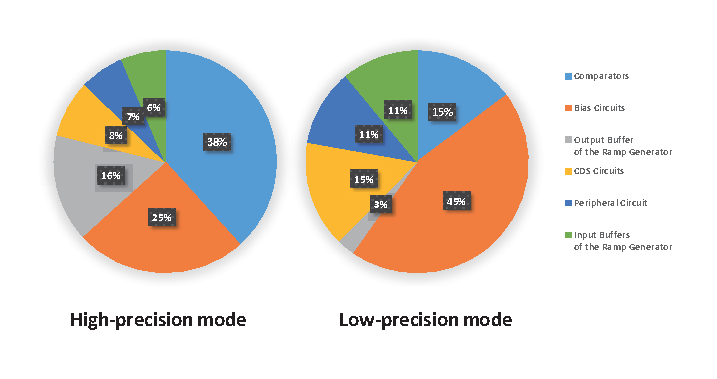
\includegraphics[width=3.5in]{./Figures/SSResults1.eps}}
	\caption{Power Saving Results of the SS ADCs.}
	\label{SSresults1}
\end{figure}

\begin{figure}[htbp]
	\centerline{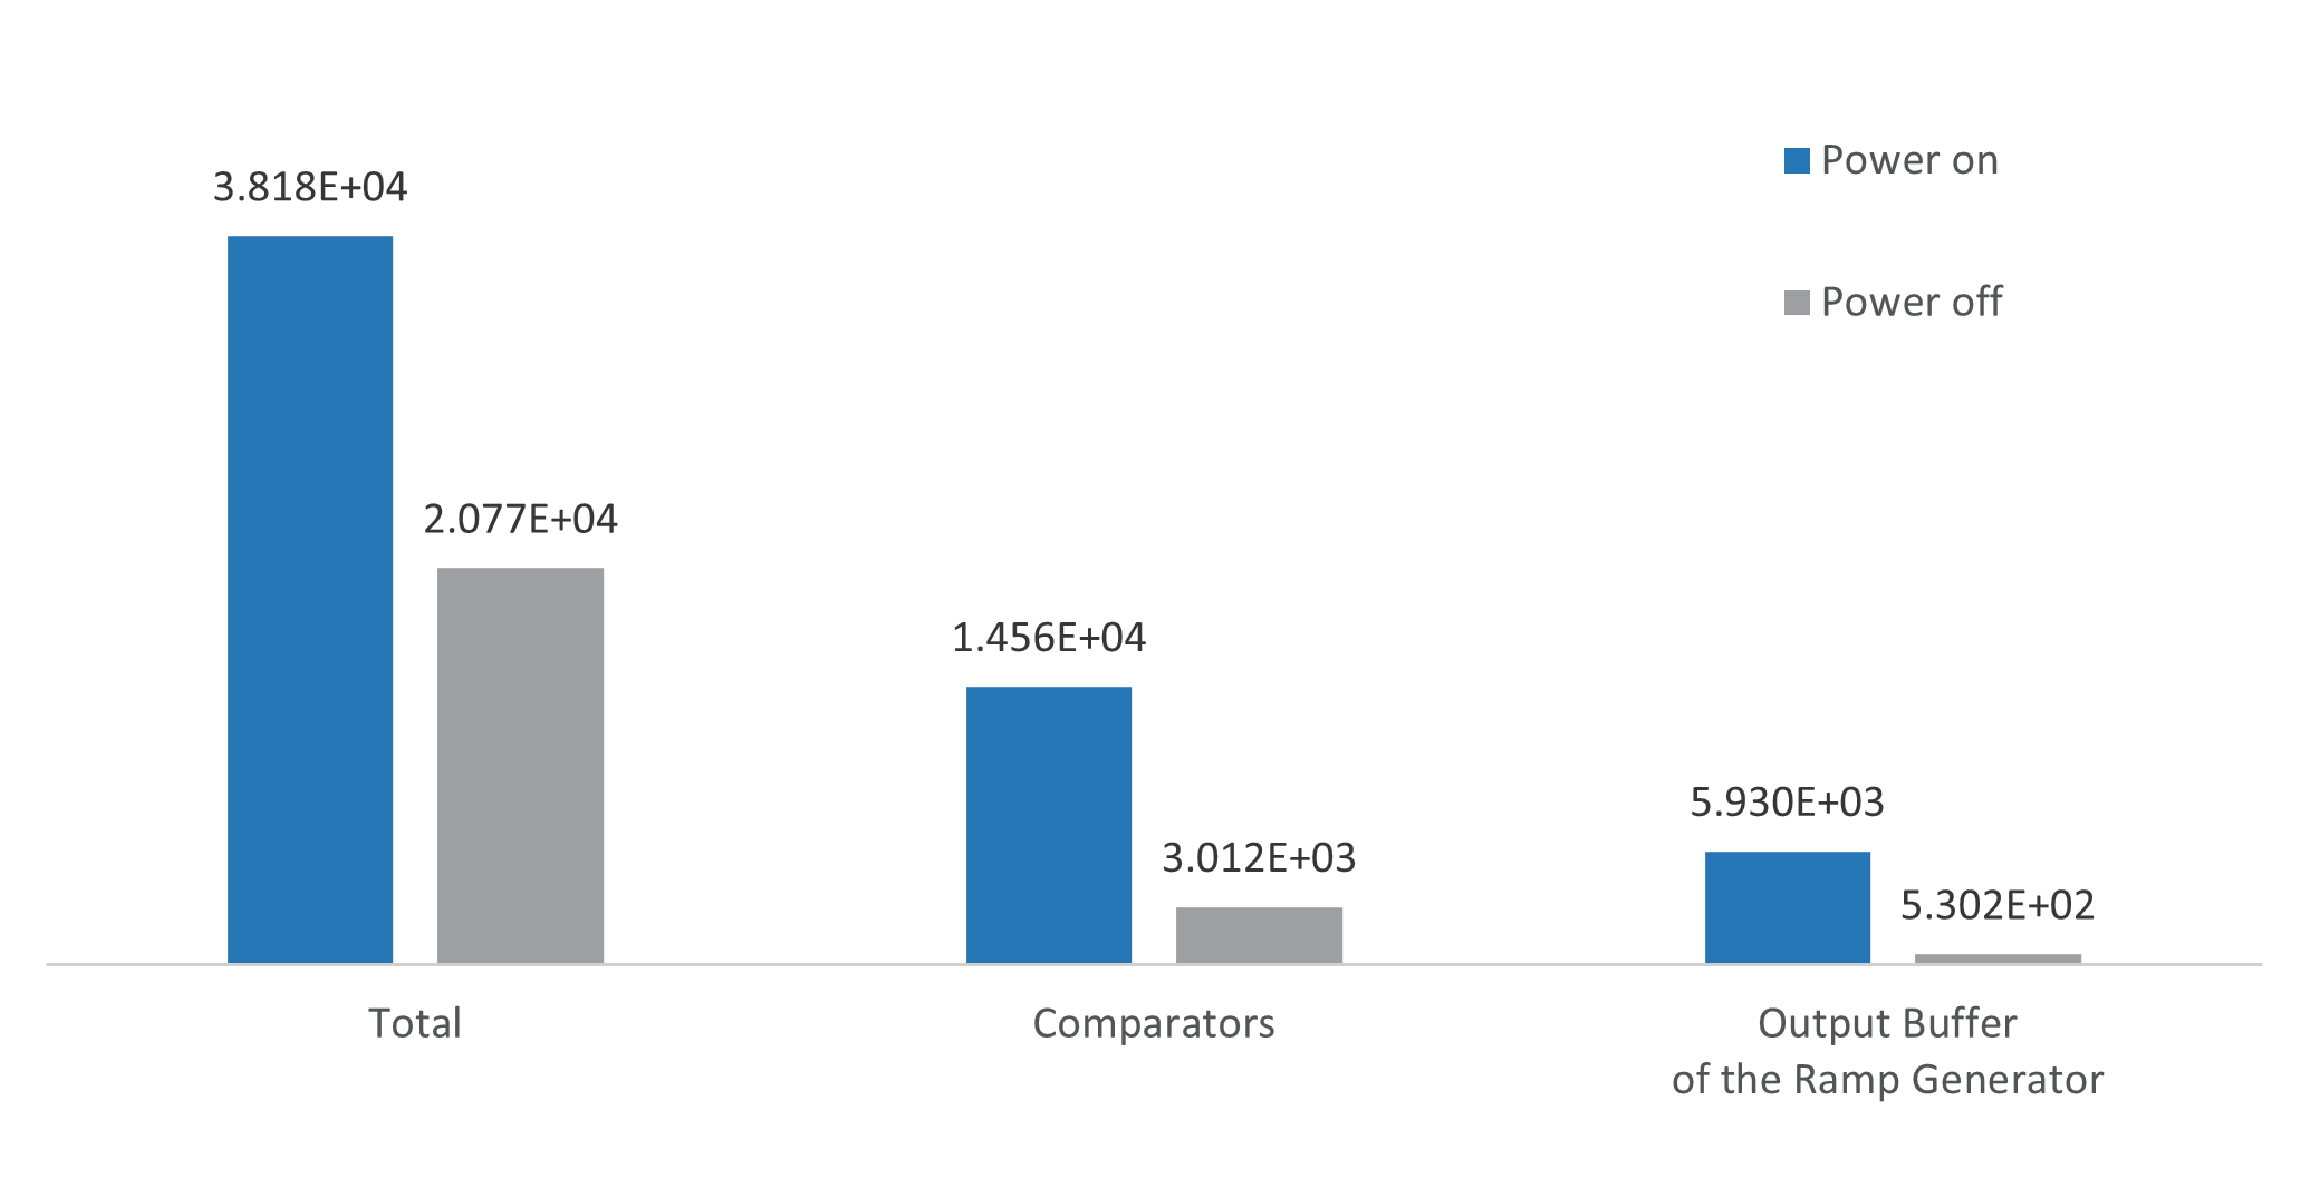
\includegraphics[width=3.5in]{./Figures/SSResults2.eps}}
	\caption{Power Saving Results of the SS ADCs.}
	\label{SSresults2}
\end{figure} 

\subsection{Evaluation of the SAR/SS ADCs}

The fundamental characteristics of the SAR/SS ADCs are summarized in Table~\ref{tab2}. 
While the throughput is set similar to the SS ADCs, fewer steps is required in the SAR/SS ADCs, where 1 conversion step counts for 2 clock periods. 
The SNDR is 24.25/57.87 dB and the ENOB is 3.74/9.32 bits, consistent with the design specifications. 
The power consumption is 256.1uW/column for high-precison conversion and 137.1uW/column for low-precison conversion, respectively. 
According to the energy analysis presented in Fig.~\ref{SARresults1}, most parts of the SAR/SS ADCs' power consumption 
are taken up by the column-parallel buffers of reference voltages in the sub-ADCs.
For low-precison conversion, the energy of the SAR/SS ADCs can also be saved to nearly half. 
The related quantity results is presented in Fig.~\ref{SARresults2}.

\begin{table}[htbp]
	\caption{Performance of the SAR/SS ADCs}
	\begin{center}
		\begin{tabular}{|c|c|}
			\hline
			\textbf{Prameter}& \textbf{Value} \\
			\hhline{|==|}
			\textbf{Process}& 65nm \\
			\hline 
			\textbf{Supply voltage}& 2.5/1.2 V \\
			\hline
			\textbf{Clock Frequency}&	20MHz \\
			\hline
			\textbf{Architecture}&	SAR/SS \\
			\hline
			\textbf{Quantization bits}&	4/10 bits \\
			\hline
			\textbf{Conversion time (us)}&	10.1us \\
			\hline
			\textbf{Number of parallel columns}&	512 \\
			\hline
			\textbf{Throughput (samples per second)}&	50.7M \\ 
			\hline
			\textbf{Power (per column)}&	137.1/256.1 uW \\
			\hline
			\textbf{SNDR}& 24.25/57.87 dB@ 10.06 kHz \\
			\hline
			\textbf{ENOB}& 3.74/9.32 bits \\
			\hline
			\textbf{FOM$^{\mathrm{a}}$}& 103.64/4.05 pJ/step\\
			\hline
			\multicolumn{2}{l}{$^{\mathrm{a}}\textbf{FOM}=(\textbf{Power}\ast \textbf{Conversion}\ \textbf{time})/2^{\textbf{ENOB}}$ }	    
		\end{tabular}
		\label{tab2}
	\end{center}
\end{table}

\begin{figure}[htbp]
	\centerline{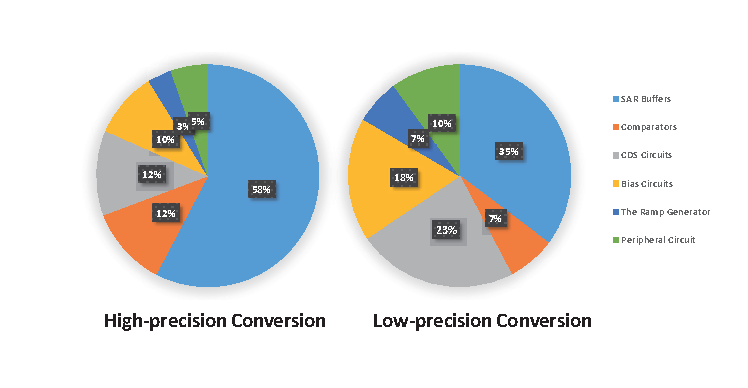
\includegraphics[width=3.5in]{./Figures/SARResults1.eps}}
	\caption{Power Saving Results of the SAR/SS ADCs.}
	\label{SARresults1}
\end{figure} 

\begin{figure}[htbp]
	\centerline{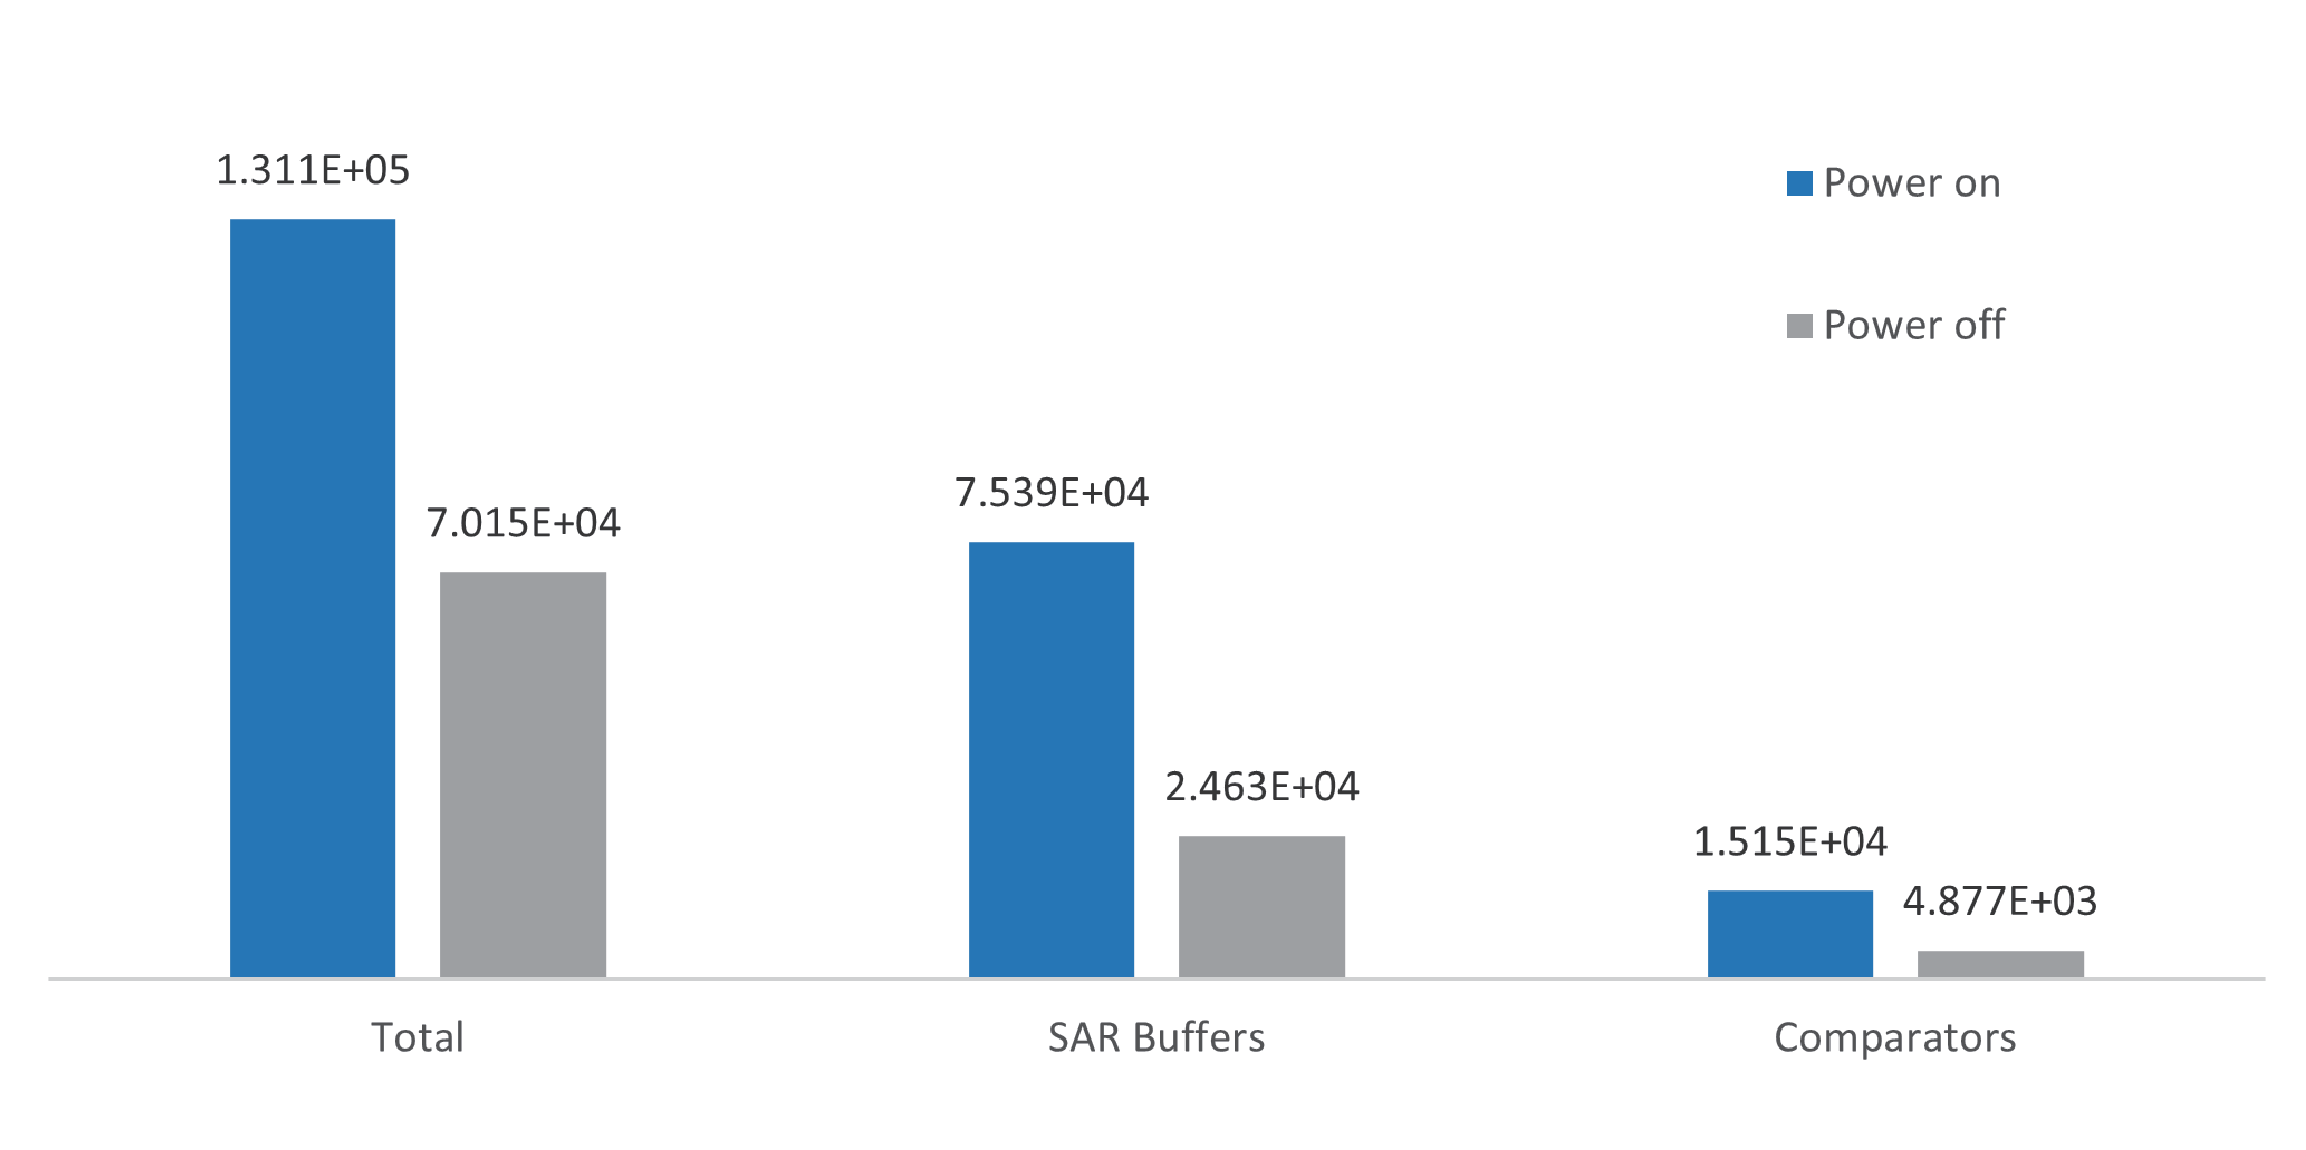
\includegraphics[width=3.5in]{./Figures/SARResults2.eps}}
	\caption{Power Saving Results of the SAR/SS ADCs.}
	\label{SARresults2}
\end{figure} 

\section{Discussions}\label{discussion}
Combining precision adaptive and power gating strategies, both the SS ADCs and SAR/SS ADCs can save energy dynamically and significantly. 
It is because that in the column-parallel and SS-logic-adopted ADCs, not only a large amount of currents can be under control but also the power gated time can be rather long. 

In comparison, the SAR/SS ADCs can support higher quantization bits and require fewer extra control circuits for the adaptive precision, 
while SS ADCs inherently require less area and can effectively applied in the 4/8-bit situation. 
Therefore, according to specific design specifications, different structures can be chosen. 

For other different precision configurations (e.g. 2/8 adaptive precision) and number of parallel collumns, 
the corresponding power consumption and energy-saving performance can also be estimated with extending the evaluation results in Sect.~\ref{result}. 

\section{Conclusions}\label{conclusion}

In this work, a method combining adaptive precision and fine-grained power gating strategies is proposed for column-parallel ADC design. 
According to the evaluation results of two CIS-applied ADC designs, almost a half of the ADCs’ power consumption can be reduced for low-precision conversion, 
while just a few of extra control circuits is required.

The method in this paper may resonate with varying downstream algorithms, especially powerful NN models, for efficient multi-tasks analysis. 
As such an integrated system will be promising for more intelligent edge computing in the future, further works on the co-design of ADCs and NNs remain to be developed.

\bibliographystyle{IEEEtran}
\bibliography{ADCpaper}

\end{document}
